\section{Arquitectura del Sistema}

\subsection{Vista Física}

\begin{figure}[H]
    \centering
    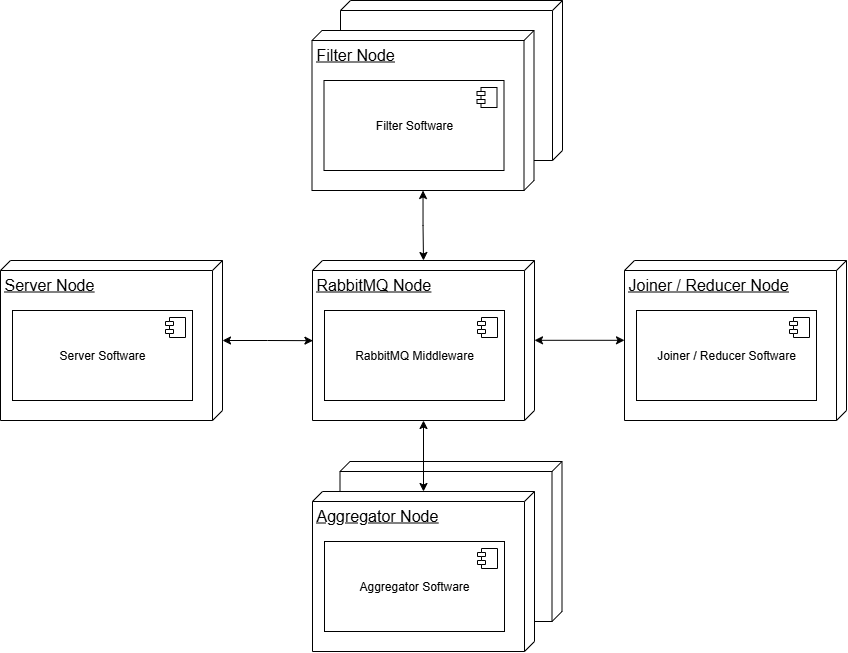
\includegraphics[width=0.6\textwidth]{imagenes/vistas/despliegue.png}
    \caption{Diagrama de despliegue del sistema}
    \label{fig:despliegue}
\end{figure}

\subsection{Vista Lógica}

\begin{figure}[H]
    \centering
    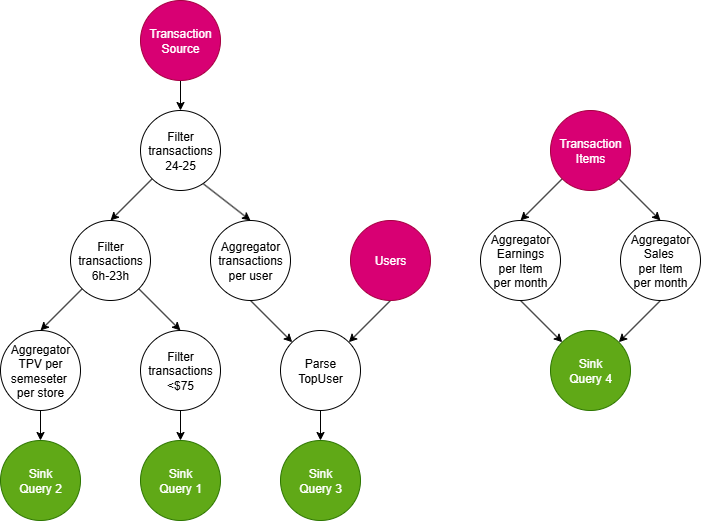
\includegraphics[width=0.6\textwidth]{imagenes/vistas/dag.png}
    \caption{Grafo acíclico dirigido (DAG) representando las tareas del sistema}
    \label{fig:dag}
\end{figure}

\newpage
\begin{figure}[H]
    \centering
    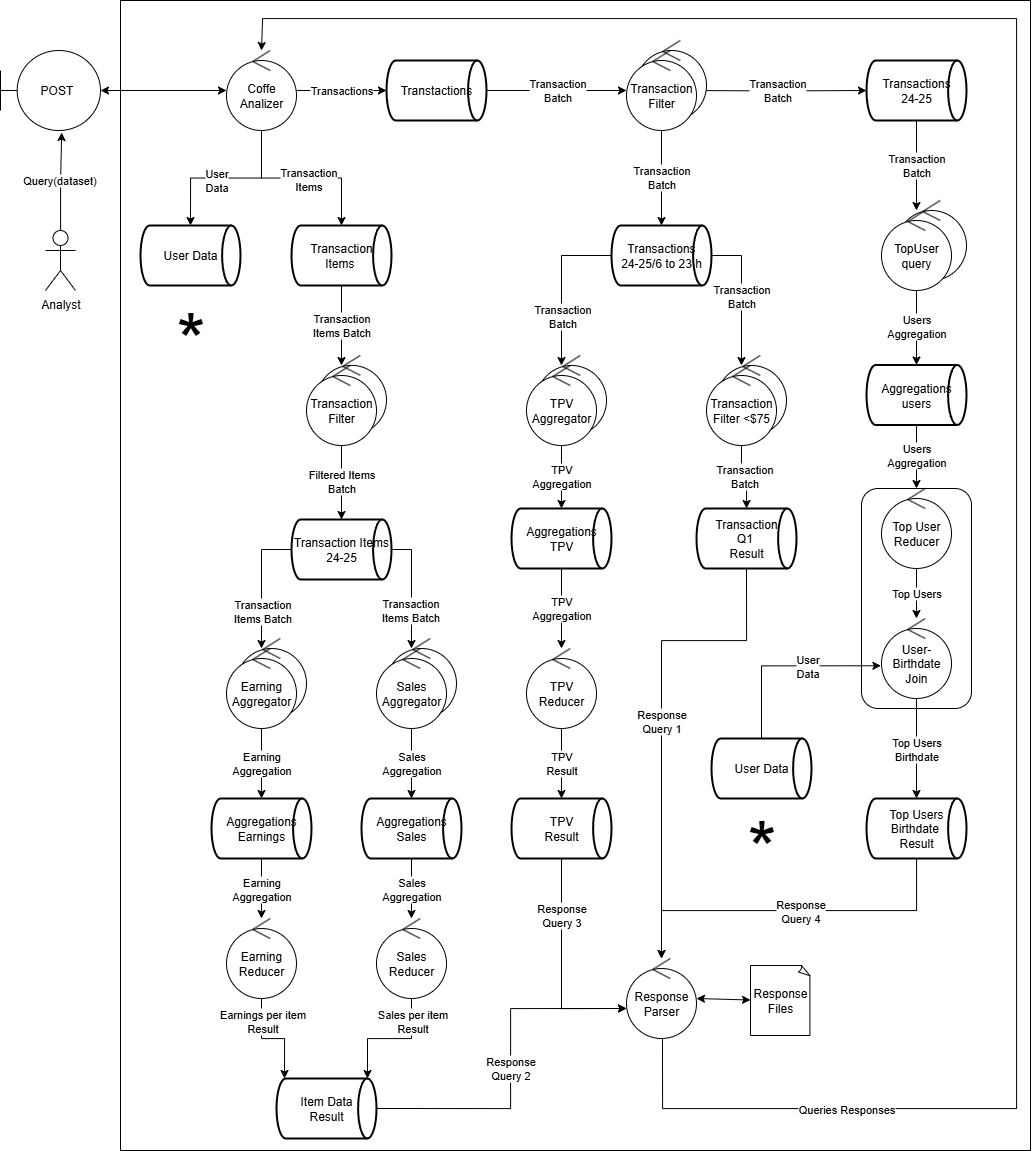
\includegraphics[width=1\textwidth]{imagenes/vistas/robustez.png}
    \caption{Diagrama de robustez del sistema}
    \label{fig:robustez}
\end{figure}

\subsection{Vista de Procesos}

\begin{figure}[H]
    \centering
    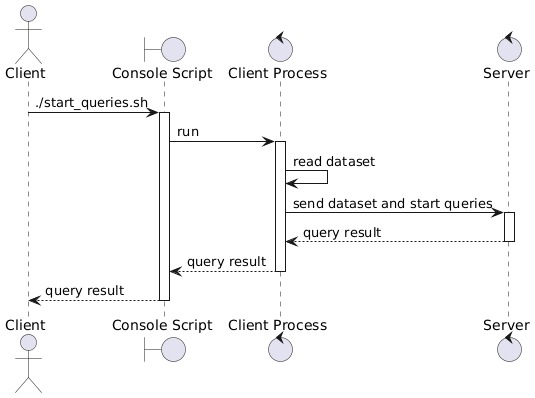
\includegraphics[width=0.8\textwidth]{imagenes/vistas/secuencia1.jpg}
    \caption{Diagrama de secuencia vista desde el cliente}
    \label{fig:secuencia1}
\end{figure}

\begin{figure}[H]
    \centering
    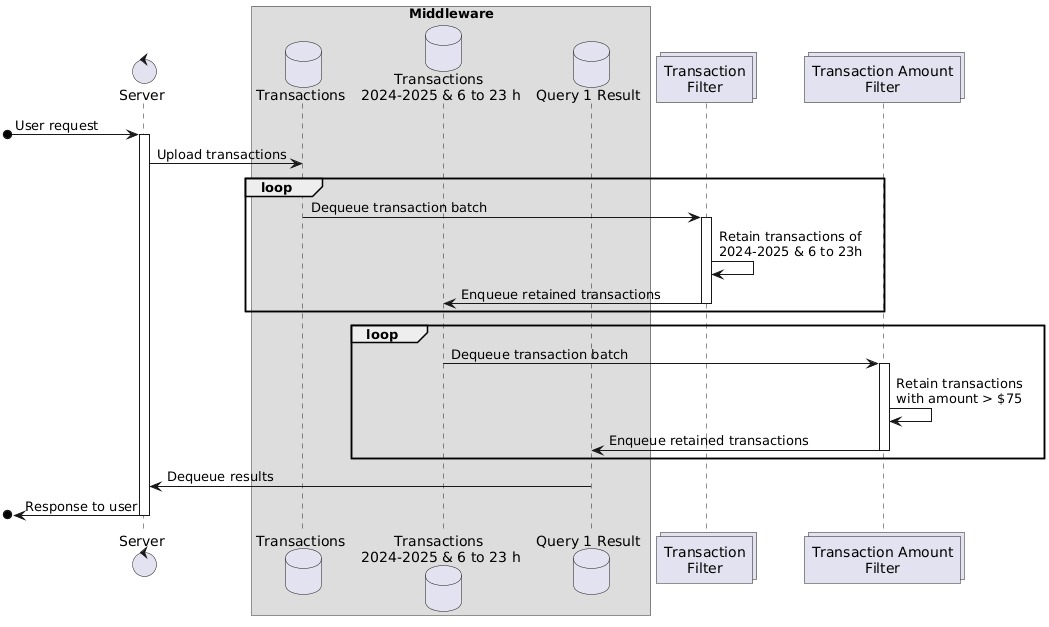
\includegraphics[width=0.8\textwidth]{imagenes/vistas/secuencia2.jpg}
    \caption{Diagrama de secuencia para la query \ref{item:query1}}
    \label{fig:secuencia2}
\end{figure}

\begin{figure}[H]
    \centering
    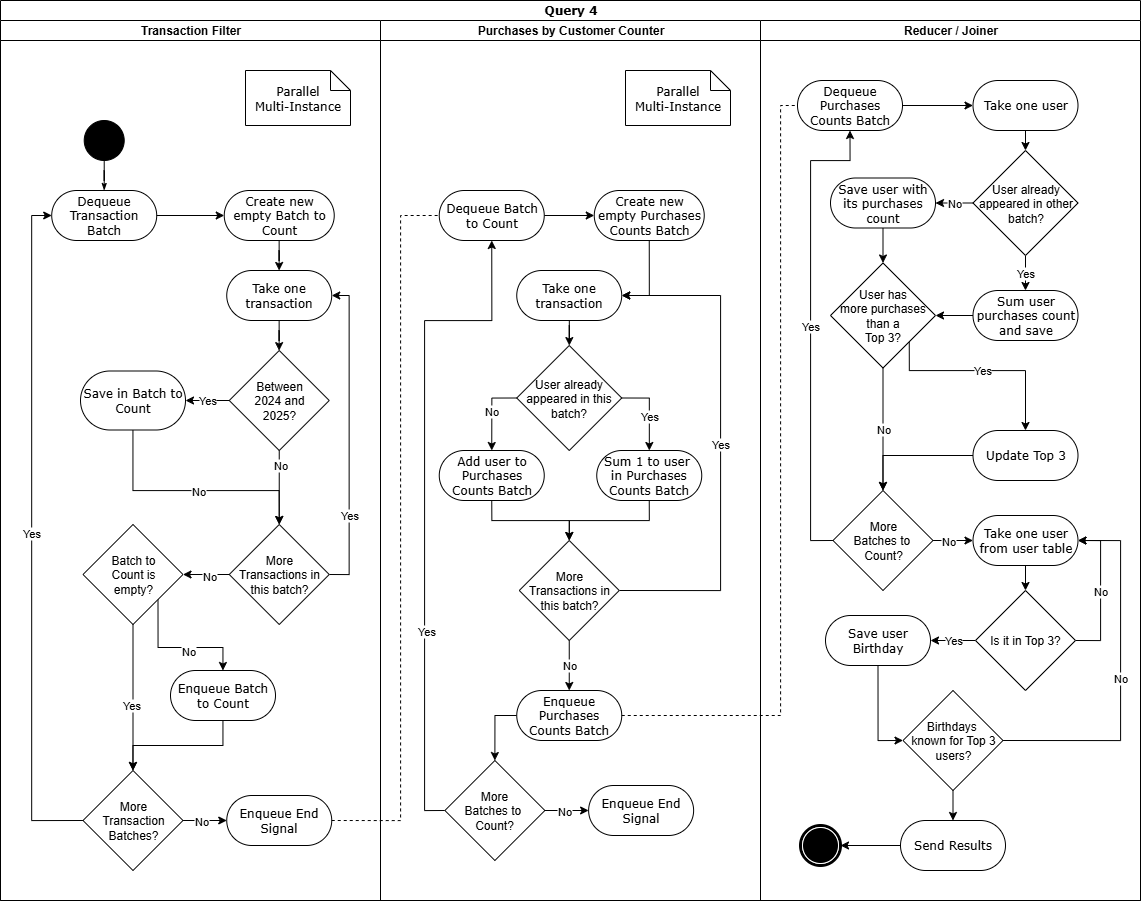
\includegraphics[width=0.8\textwidth]{imagenes/vistas/actividad.png}
    \caption{Diagrama de actividad de la query \ref{item:query4}}
    \label{fig:actividad}
\end{figure}



\subsection{Vista de Desarrollo}

\begin{figure}[H]
    \centering
    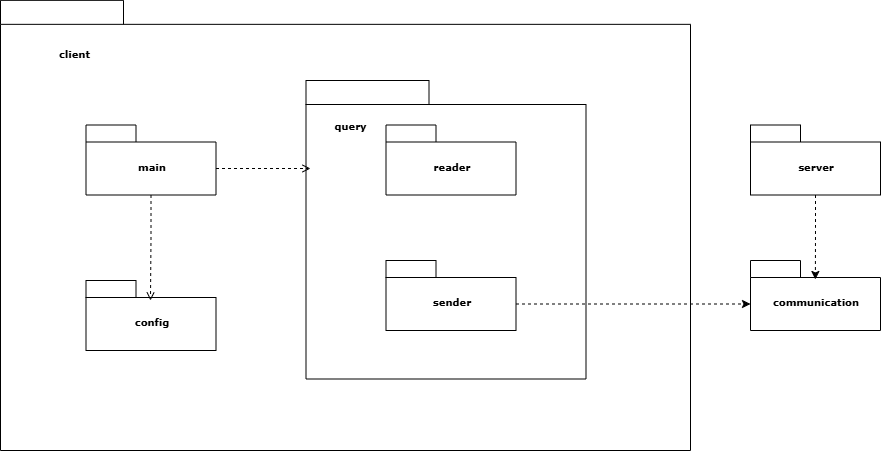
\includegraphics[width=0.8\textwidth]{imagenes/vistas/paquetes-client.png}
    \caption{Diagrama de paquetes del cliente del sistema}
    \label{fig:paquetes-client}
\end{figure}

\begin{figure}[H]
    \centering
    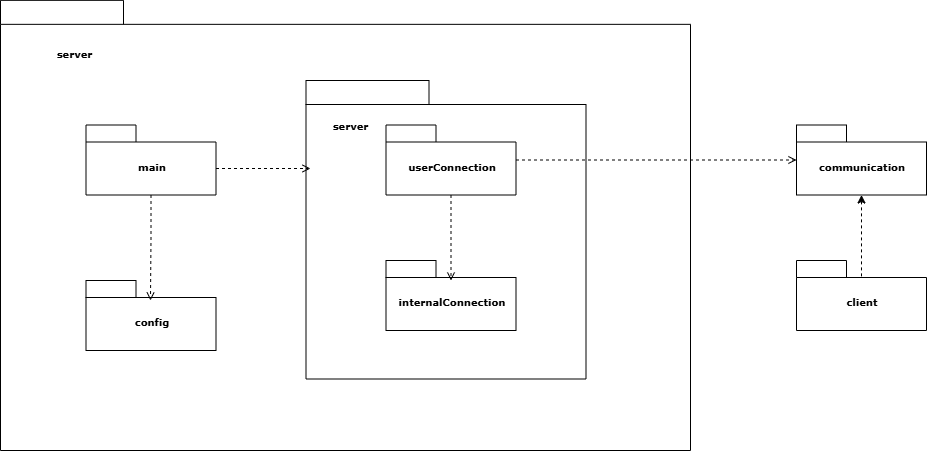
\includegraphics[width=0.8\textwidth]{imagenes/vistas/paquetes-server.png}
    \caption{Diagrama de paquetes del servidor del sistema}
    \label{fig:paquetes-server}
\end{figure}

\begin{figure}[H]
    \centering
    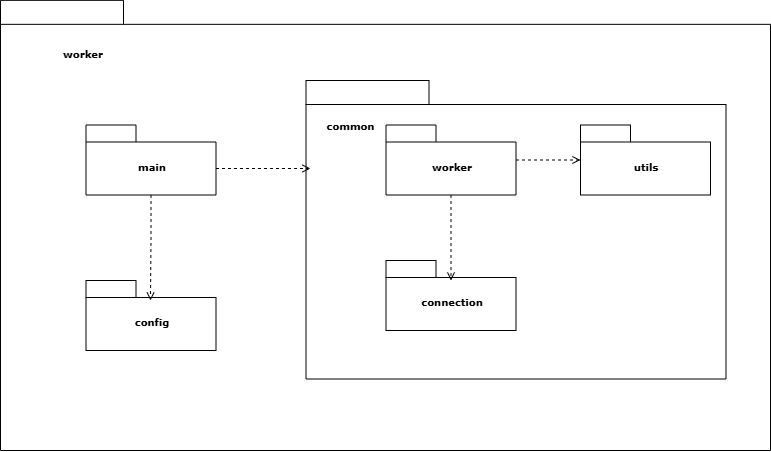
\includegraphics[width=0.8\textwidth]{imagenes/vistas/paquetes-workers.png}
    \caption{Diagrama de paquetes de los workers del sistema}
    \label{fig:paquetes-workers}
\end{figure}